\section{Integrationstest}
Integrationstests udføres for at checke om de enkelte software moduler passer sammen. Man integrationstester software pakker, klasser og subsystemer\todo{hvad er subsystemer helt konkret?}.

\subsection{Før integrationstest}
Før man begynder at integrationsteste er der nogle ting som man bør have opfyldt:
\begin{itemize}
	\item Unittests skal være færdige. Dette gælder for samtlige metoder!
	\item Systemets dependancy tree skal være kendt! jf. ATM opgaven.
	\item Integrationstesten er planlagt.
\end{itemize}

\subsection{Typer af integrationstest}
Der findes flere typer af tilgange til at integrationsteste.

Først lidt om dependancy trees. \todo{Skriv om dependancy trees + paralleler til ATM projektet}

\subsubsection{Big Bang testing}

\paragraph{Hvorfor Big Bang testing?}

\paragraph{Hvorfor ikke Big Bang testing?}

%%%%%%%%%%%%%%%%%%%%%%%%%%%%%%%%%%%%%%%%%%%%%%%%%%%%%%%%%%%%%%%%%%%%%%%%%%%%%%%%%%%%%%%%%%%%%%%%%%

\subsubsection{Bottom-Up testing}

\begin{itemize}
	\item Starter i bunden af dependancy træet - nederste lag testes først.
\end{itemize}

\begin{figure}
\centering
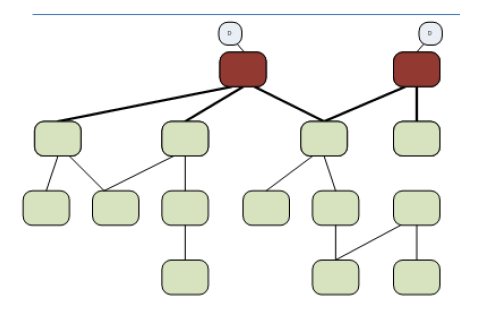
\includegraphics[width=0.7\linewidth]{figs/bottomUp.PNG}
\caption{Illustration af Bottom-Up testing.}
\label{fig:bottomUp}
\end{figure}

\paragraph{Hvorfor Bottom-Up testing?}

\paragraph{Hvorfor ikke Bottom-Up testing?}

%%%%%%%%%%%%%%%%%%%%%%%%%%%%%%%%%%%%%%%%%%%%%%%%%%%%%%%%%%%%%%%%%%%%%%%%%%%%%%%%%%%%%%%%%%%%%%%%%%

\subsubsection{Top-Down testing}

\begin{itemize}
	\item Starter i toppen af dependancy træet - øverste lag testes først.
\end{itemize}

\begin{figure}
\centering
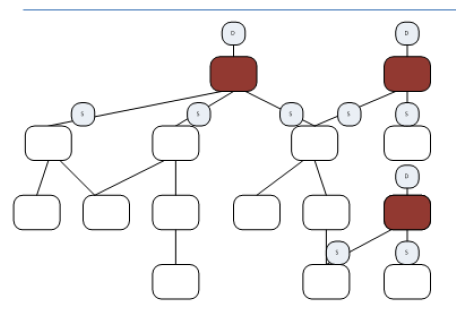
\includegraphics[width=0.7\linewidth]{figs/topDown.PNG}
\caption{Illustration af Top-Down testing.}
\label{fig:topDown}
\end{figure}

\paragraph{Hvorfor Top-Down testing?}

\paragraph{Hvorfor ikke Top-Down testing?}

%%%%%%%%%%%%%%%%%%%%%%%%%%%%%%%%%%%%%%%%%%%%%%%%%%%%%%%%%%%%%%%%%%%%%%%%%%%%%%%%%%%%%%%%%%%%%%%%%%

\subsubsection{Collaboration testing}

\begin{itemize}
	\item I collaboration test tager man en "gren" ad gangen i dependency træet.
\end{itemize}

\begin{figure}
\centering
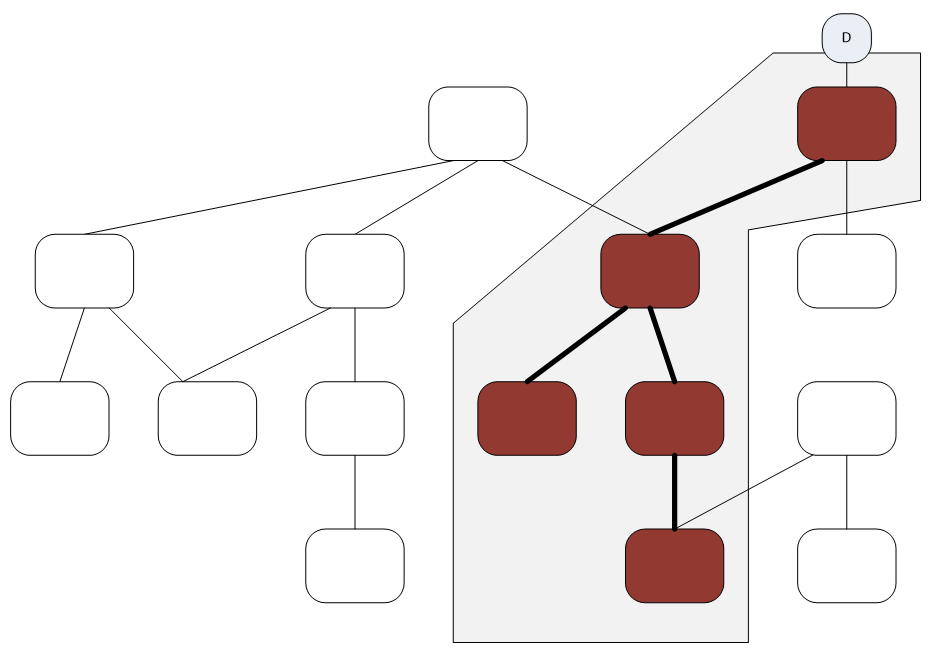
\includegraphics[width=0.7\linewidth]{figs/collaborationTesting.PNG}
\caption{Illustration af Collaboration testing.}
\label{fig:collaborationTesting}
\end{figure}

\paragraph{Hvorfor Collaboration testing?}

\paragraph{Hvorfor ikke Collaborationp testing?}

%%%%%%%%%%%%%%%%%%%%%%%%%%%%%%%%%%%%%%%%%%%%%%%%%%%%%%%%%%%%%%%%%%%%%%%%%%%%%%%%%%%%%%%%%%%%%%%%%%

\subsubsection{Sandwich testing}

\begin{figure}
\centering
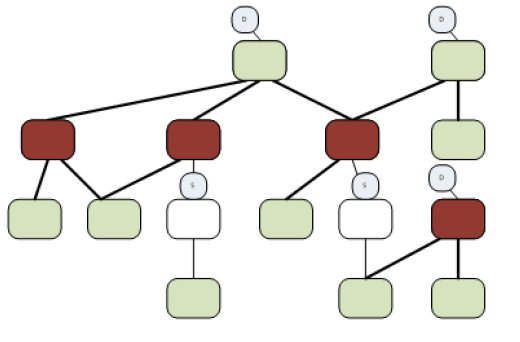
\includegraphics[width=0.7\linewidth]{figs/sandwich.PNG}
\caption{Illustration af Sandwich testing.}
\label{fig:sandwich}
\end{figure}

\paragraph{Hvorfor Sandwich testing?}

\paragraph{Hvorfor ikke Sandwich testing?}